\section{Experimental Results}

Our experimental system configurations are follows.
\begin{itemize}
	\item System: Intel i7-2600 with 8 cores and 16GB memory,
	\item OS: Linux kernel 4.5 with stream assignment support,
	\item SSD: Samsung PM963 480GB with internal stream support,
\end{itemize}

For an objective evaluation, we compared \textsf{\small PCStream} with three
existing schemes: \textsf{\small Baseline}, \textsf{\small ManualStream}\footnote{For brevity, 
we denote the manual allocation method used in ~\cite{MultiStream} by 
\textsf{\small ManualStream}}~\cite{MultiStream}, and
\textsf{\small AutoStream}~\cite{AutoStream}.  \textsf{\small Baseline} stands for a legacy
SSD that does not support a multi-stream feature. \textsf{\small ManualStream} represents
is manually optimized for multi-streamed SSDs.
\textsf{\small AutoStream} is an LBA-based data separation technique which is
implemented at the device driver layer. 

The SSD we used supports up to 9 streams; eight NVMe standard compliant streams
and one default stream. If a write command does not specify its stream ID,
it is writtne to the default stream.
Furthermore, we modified the SSD firmware to implement internal streams.
Additional DRAM space is used to hold data structures for internal streams 
and GC behavior is changed to copy valid pages to dedicated internal streams.
We also implemented new commands using an \texttt{nvme-cli} tool to get several 
device internal information, such as the WAF or the valid time of data in every blocks, 
for the detailed analysis.

For various workloads, we have used RocksDB and Cassandra for append-only workload,
SQLite for in-place update, GCC for write-once pattern, and combinations of couple 
of workloads.
To warm up the device, the SSD was filled about 90\% of the capacity.
RocksDB and Cassandra runs Yahoo! Cloud Serving Benchmark (YCSB)~\cite{YCSB} 
with 120,000,000 keys.
In theory, both applications are based on LSM-tree so
mainly have 3 kinds of data types as analyzed in Section 3.
However, we identified about 5 PCs during runtime and we consider
the extra PCs as management use.
SQLite runs TPC-C~\cite{TPCC} with 20 warehouses. 
Similarly, SQLite has 2 kinds of data types in theory
but we identified 4 PCs.
GCC compiles kernel source 30 times where randomly chosen 1/3 of source files
are modified for the each run.
For mixed workload, we ran RocksDB and compile scenario together for Mixed 1,
and SQLite and compile scenarios for Mixed 2.
Since GCC writes many kinds of temporary files as well as
long-lived files, GCC has more than 20 PCs which makes
clustering process effective for the GCC and mixed workloads.


\subsection{WAF Comparison}

\begin{figure}[t]
	\centering
	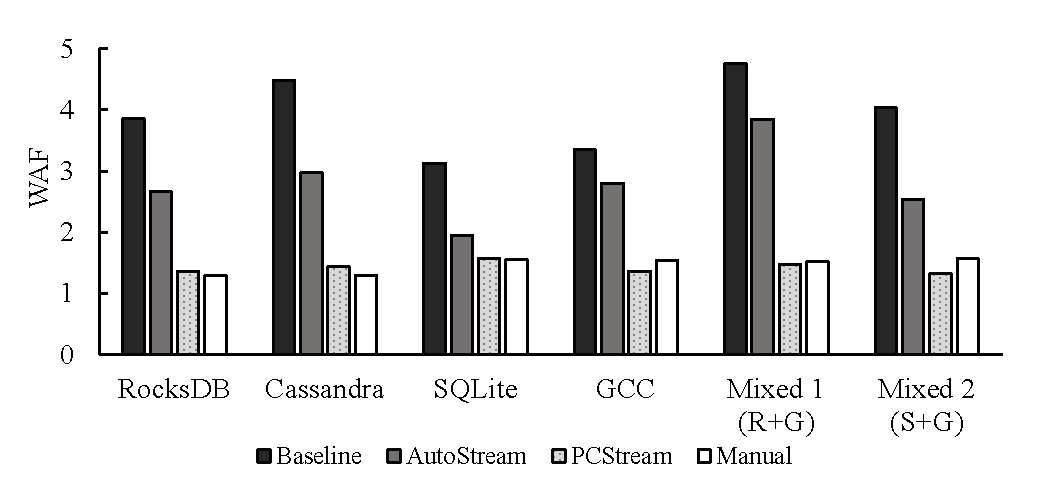
\includegraphics[width=0.9\linewidth]{figure/WAF}
	\caption{The WAF comparison for various workloads.}
	\label{fig:waf}
	%\vspace{-36pt}
\end{figure}


We compared WAF of the existing techniques with \textsf{\small PCStream} for 
various workloads and the result is shown in Fig.~\ref{fig:waf}.  
\textsf{\small PCStream} was quite effective in reducing WAF, 
thus achieving an equivalent level of the WAF reduction as in \textsf{\small Manual}.  
For example, \textsf{\small PCStream}  
reduced WAF by 63\% over \textsf{\small Baseline} on average.
\textsf{\small PCStream} also outperformed \textsf{\small AutoStream} 
by reducing WAF by 49\% on average.
The result shows that separating short-lived data (e.g., log or temp files) 
from long-lived one (e.g., compaction or result files) 
using PC was quite effective in reducing WAF.  
Moreover, \textsf{\small PCStream} even showed similar WAF to \textsf{\small Manual}, 
reducing it by up to 69\% over \textsf{\small AutoStream} for \texttt{Mixed 1} case.

AutoStream was not able to achieve high WAF reduction because of 
the lack of relationship between hotness and address in the general I/O workloads.
As a result, AutoStream showed WAF larger than 2 for all the cases except SQLite.
Only SQLite has in-place update pattern for log files, but the larger amount of data are
written for database files whose lifetimes are determined by the client
which makes hard to predict their lifetime by the address.
In PCStream, however, long-lived data in database files are moved to internal streams
during GC so that we can further reduce WAF.

For GCC and mixed workloads, PCStream achieved even better than Manual
since the Manual scheme has static stream allocation.
In Manual, once data types is mapped to the stream, the mapping is not changed 
during runtime.
For complex workloads which have large number of PCs such as mixed cases,
it is difficult to expect data lifetimes in detail based on the data types.
If the lifetime pattern is changed during runtime or the programmer choose
second best stream mapping,
Manual scheme lose the potential benefit in reducing WAf.
However, the reclustering enables PCStream to adapt changing workload or find
better stream mapping.
The detailed analysis will be shown in the following subsections.

\begin{comment}
For example, both \textsf{\small PCStream} and \textsf{\small Manual} reduced WAF by 38\% over \textsf{\small Baseline} for the \texttt{UR} case. 
Compared with \textsf{\small AutoStream}, \textsf{\small PCStream} was more effective, reducing WAF more by 35\% on average.  
\textsf{\small PCStream} outperformed \textsf{\small AutoStream} by reducing WAF by 35\% on average.
Fig. 6 also indicates that the two-phase stream assignment technique is effective.  
\textsf{\small PCStream} outperformed \textsf{\small PCStream$^{*}$} by 12\% on average in the WAF reduction.
As shown in Fig. 6, \textsf{\small PCStream$^*$} reduced WAF by up to 30\% over \textsf{\small AutoStream}.  
\end{comment}

\subsection{Per-stream Lifetime Distribution}

\begin{figure}[t]
	\centering
	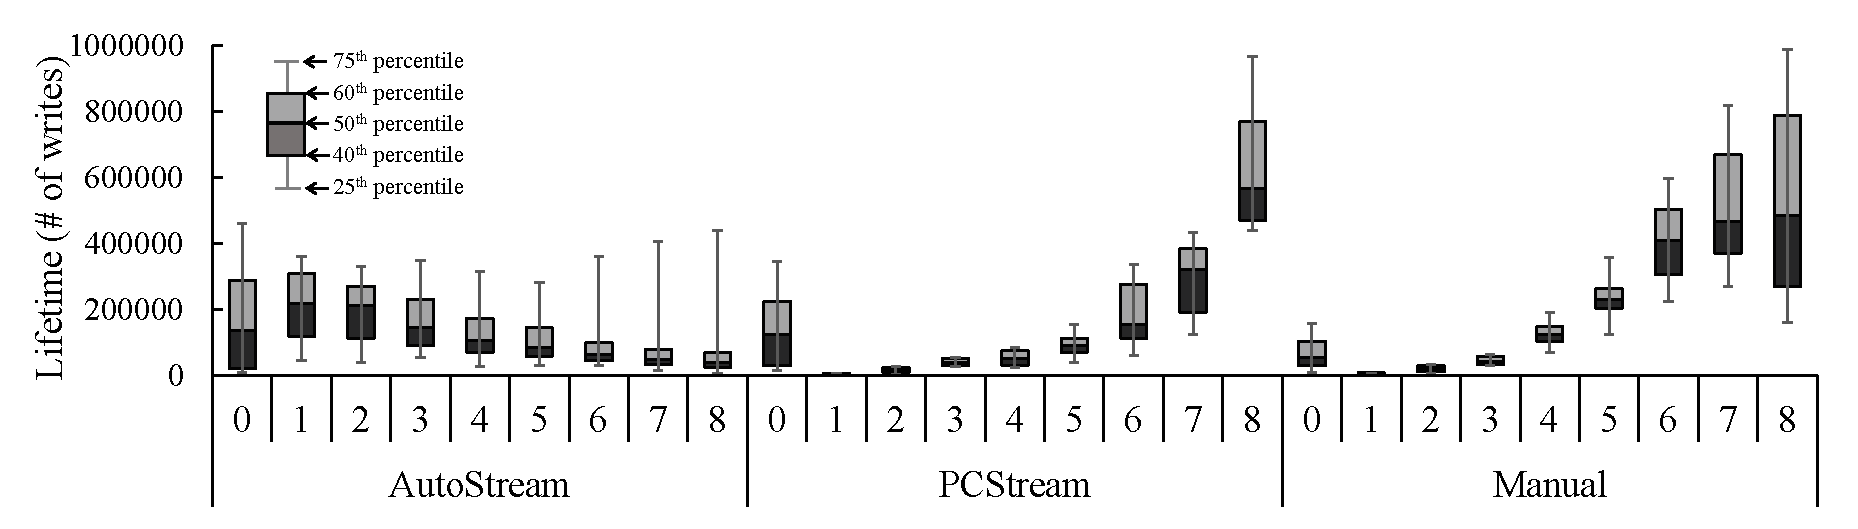
\includegraphics[width=1\linewidth]{figure/distribution}
	\caption{A Comparison of lifetime distributions of the smaller variance streams.}
	\label{fig:distribution}
	%\vspace{-36pt}
\end{figure}

In order to better understand how \textsf{\small PCStream} achieved a high reduction in WAF, 
we measured per-stream lifetime distributions under each 
technique for the \texttt{Mixed 1} scenario.
Fig.~\ref{fig:distribution} shows a box plot of data lifetimes from the 
25th percentile to the 75th percentile.
As shown in Fig.~\ref{fig:distribution}, 
streams in both \textsf{\small PCStream} and Manual are divided into two groups, 
$G1$ = $\{$1, 2, 3, 4, 5$\}$ and $G2$ = $\{$6, 7, 8$\}$, 
where $G1$ includes streams with short lifetimes and small variances 
(i.e., streams 1, 2, 3, 4, and 5) 
and $G2$ includes streams with large lifetimes and large variances (i.e., streams 6, 7, and 8).  
In PCStream, every streams especially streams in G2 showed smaller variance than 
Manual.
This is because long-lived data in those streams are moved to internal streams, thus 
reducing the lifetime variance.
Since the GC copy cost is affected by how data in $G1$ and $G2$ are mixed into the same block, 
\textsf{\small PCStream} can significantly reduce the GC overhead 
by avoiding such data mixtures in the same block by separating $G1$ and $G2$ into different streams. 

On the other hand, AutoStream was not able to achieve small variance of data lifetimes in a stream.
AutoStream allocates data in a address range to stream 1 at first.
The data will be allocated to stream 2 when the frequency of the range hits the 
pre-defined threshold which means the address range holds hotter data.
However, since there is no strong relation between hotness of data and the address in RocksDB
or GCC workload, 
long-lived data can be placed to the hot address range which results 
very high lifetime variances for all the streams.
Since a block with very small number of valid pages will be easily involved to GC,
long-lived data in stream 8 is the worst case scenario 
for preventing valid page copies during GC.

\subsection{Impact of the Internal Stream}

To understand the impact of the
two-phase assignment, in addition, we compared each techniques
with and without using internal streams.
Since internal streams are orthogonal to the stream management technique,
internal streams can be combined with any stream management techniques.
Fig.~\ref{fig:internal} shows the WAF comparison on the internal stream usage 
for various workloads.
Although every technqiue can benefit from using internal streams,
its effect is limited for cases other than PCStream.
Since internal streams can not help data copies from the first phase,
Baseline, where different lifetimes of data 
are allocated in a random fashion, still showed high WAF even internal streams are used.
As shown in Fig.~\ref{fig:internal}, the WAF for Baseline with internal streams is still 
larger than 2 because of the page copies from the first phase.
Similarly, for AutoStream, the benefit of internal stream was marginal 
because it can not prevent writing long-lived data to the stream of short-lived data.
Unlike other techniques, since PCStream can effectively separate short-lived data
from the first phase, we can achieve lower WAF.


\begin{figure}[t]
	\centering
	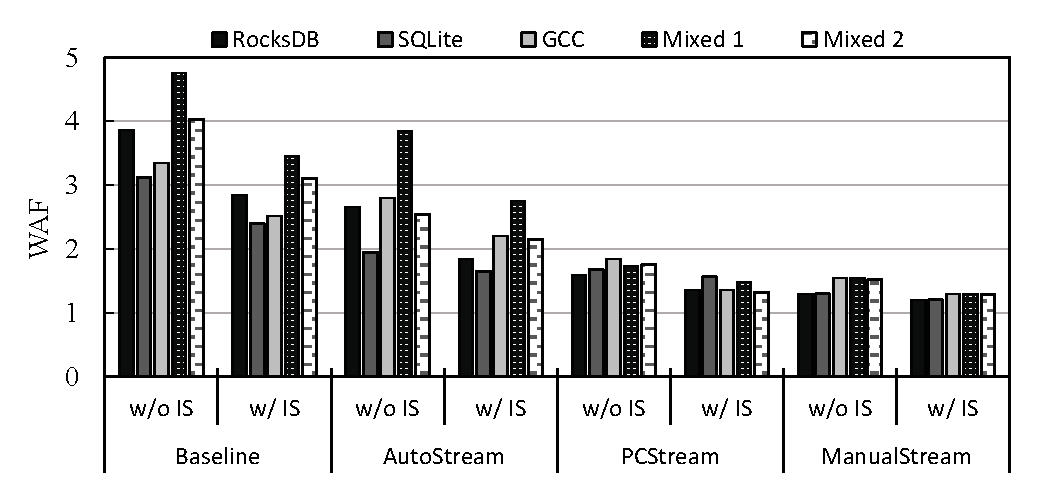
\includegraphics[width=0.9\linewidth]{figure/internal}
	\caption{An WAF comparison with and without using internal streams.}
	\label{fig:internal}
	%\vspace{-36pt}
\end{figure}


\subsection{Impact of PC-stream table}

\begin{figure}[t]
	\centering
	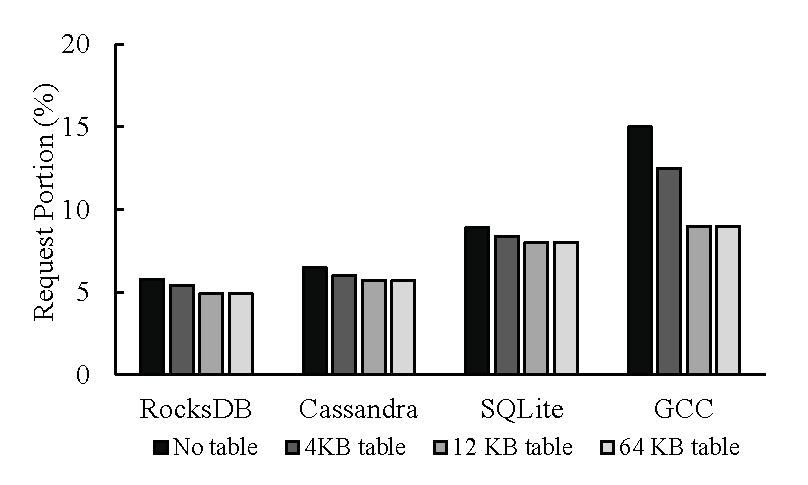
\includegraphics[width=0.7\linewidth]{figure/pctable}
	\caption{Request portion comparison of stream 0 with PC-stream table.}
	\label{fig:pctable}
	%\vspace{-36pt}
\end{figure}

As explained in Section 5, PCStream can benefit from the uniqueness of PCs
by using the PC-stream table.
PCs of frequently launched and terminated process can be directly allocated without
waiting for sufficient lifetime values are collected.
Fig.~\ref{fig:pctable} shows the request portion of stream 0, where 
awaiting requests are allocated.
Except GCC, DB applications run continuously so the benefit of using PC-stream table
was very small. 
However, since GCC is executed repeatedly, 6 percent of requests are directly
allocated to the desinated streams based on the lifetime information from the 
previous execution. 
Thanks to the direct allocation with PC-stream table, WAF was reduced from 1.96 to 1.54
for GCC workload.


